\level{2}{Dashboard APS}
	La \insglo{dashboard} è un esempio d'uso di \insglo{Norris}: rappresenta un modo in cui il \insglo{prodotto} può essere utilizzato. Essa, dunque, è una pagina web generata in automatico dal \insglo{server} \insglo{Norris}. Essa è costituita da più grafici che l'utente finale potrà visualizzare sul proprio \insglo{browser}. Di seguito viene fornito un \insglo{mockup} della pagina, che mostra a grandi linee come sarà visualizzata la \insglo{dashboard} una volta completata..
	\begin{figure}[H]\centering
        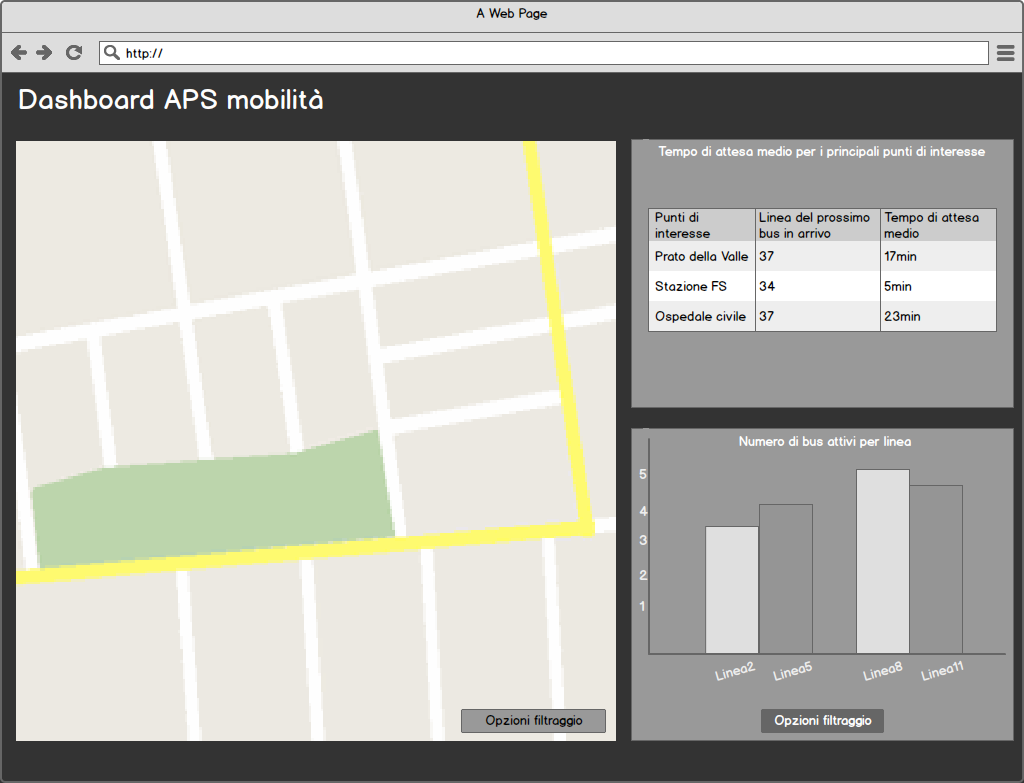
\includegraphics[width=\textwidth]{SpecificaTecnica/Pics/DashboardMockup}
        \caption{Mockup della dashboard APS}
    \end{figure}
    Vengono ora descritti i vari componenti di cui è fatta la pagina, ovvero vengono descritti i grafici che sono stati inseriti all'interno del \insglo{mockup} mostrato in precedenza.
    \level{3}{Descrizione delle componenti della Dashboard}
    	\level{4}{Map chart}
    		Tramite questo grafico l'utilizzatore della \insglo{dashboard} è in grado di visualizzare in tempo reale la posizione di tutti i bus attivi nelle varie linee dell'\insglo{APS}. Tale grafico mette inoltre a disposizione dell'utente delle opzioni riguardanti il filtraggio delle linee presenti: infatti, esso permette di scegliere le linee che si intendono visualizzare, semplicemente nascondendo e ignorando le rimanenti. In questo modo si può trasformare un grafico potenzialmente caotico (a causa della grande quantità di punti presenti al suo interno) in un molto più comprensibile e consultabile.
    	\level{4}{Table}
    		%Tale grafico è dedicato ai punti di maggior interesse di Padova. Esso fornisce all'utente utilizzatore della \insglo{dashboard} il tempo necessario all'arrivo degli autobus in alcune fermate \insglo{APS} molto frequentate. In particolare, è possibile visualizzare quanto tempo manca all'arrivo del prossimo autobus in una determinata stazione, e a quale linea il suddetto autobus appartiene. Grazie ad esso gli utenti sono in grado di capire quanto devono attendere mediamente prima di poter salire su uno dei mezzi da loro scelti.
    	%\level{4}{Bar chart}
    		Questo grafico permette all'utilizzatore della \insglo{dashboard} di visualizzare quanti autobus sono attivi su ciascuna linea dell'\insglo{APS}. Grazie a questo grafico, l'utente può ottenere utili informazioni su quanto una linea è frequentata e sul tempo di attesa che mediamente passa tra l'arrivo di un mezzo e del successivo.
    \level{3}{Creazione della Dashboard}
        In questa sezione viene mostrato quali sono i passi principali che l'utilizzatore di \insglo{Norris} deve fare per creare la \insglo{Dashboard} \insglo{APS}. La descrizione che segue può essere maggiormente compresa grazie al diagramma delle attività qui presente.
        \begin{figure}[H]\centering
            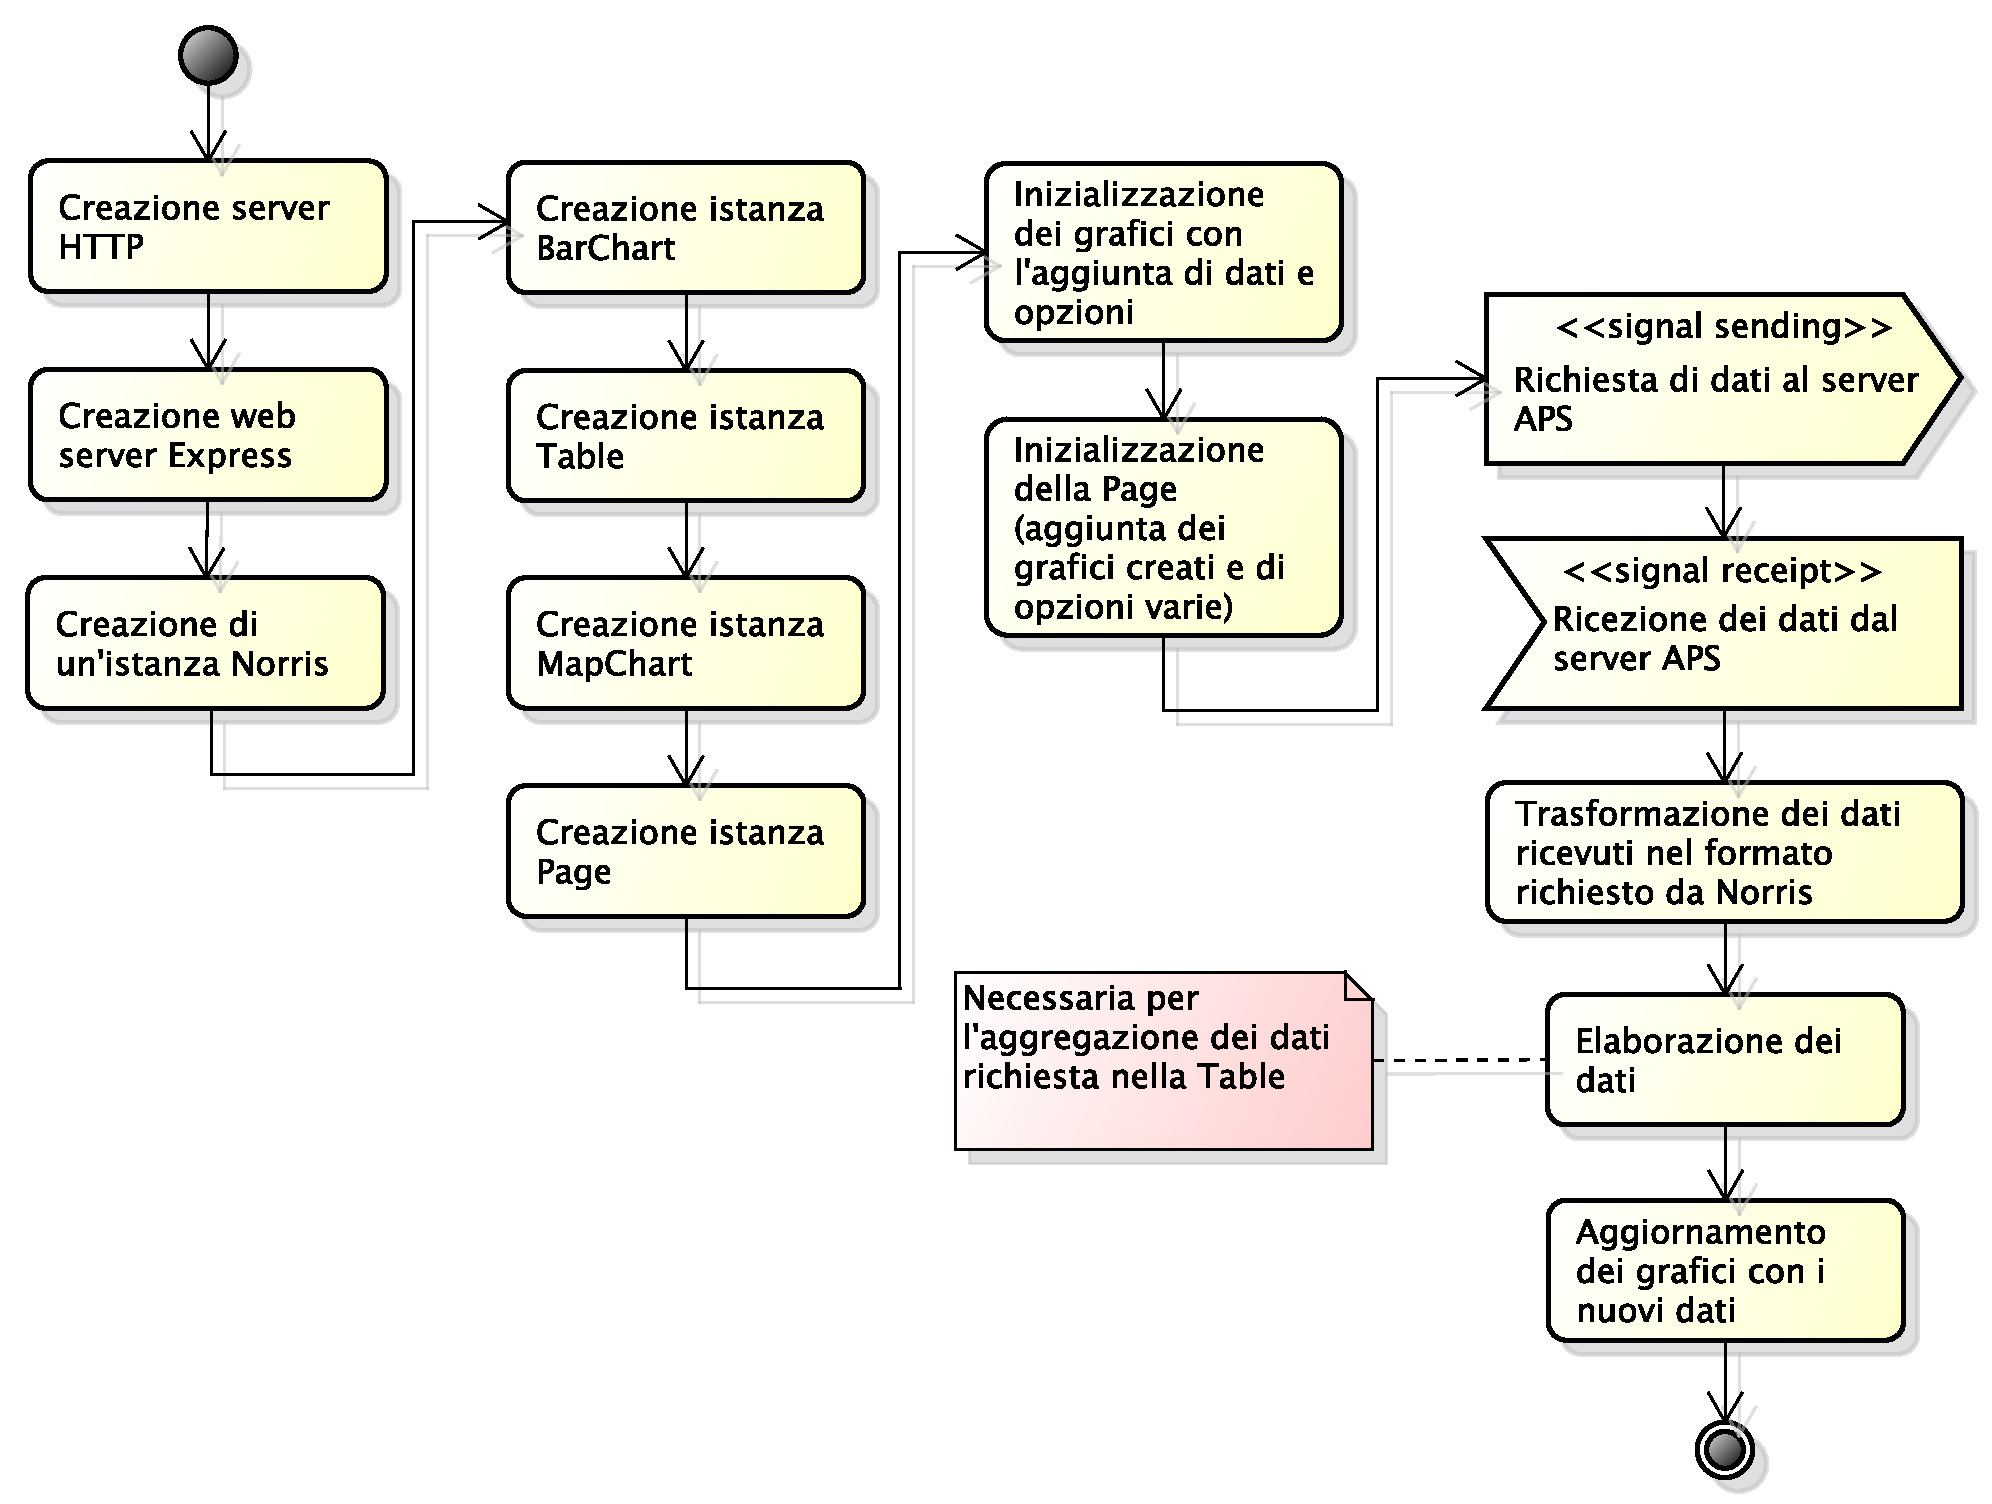
\includegraphics[width=\textwidth]{SpecificaTecnica/Pics/CreateDashboard.pdf}
            \caption{Creazione della Dashboard - diagramma delle attività}
        \end{figure}
        \begin{enumerate}
            \item Requisito fondamentale per la creazione della \insglo{dashboard} è che esista e sia correttamente funzionante un'istanza di \insglo{Norris}. Dunque, seppur banale, la prima cosa che l'utilizzatore di \insglo{Norris} deve fare è assicurarsi di ciò.
            \item In secondo luogo vanno creati i grafici che dovranno essere contenuti nella pagina web. Essi inizialmente sono vuoti (sono privi di impostazioni e di dati, che verranno aggiunti successivamente). Lo sviluppatore fa uso dell'interfaccia \texttt{Norris::InternalAPIManager::Norris} per fare ciò. Essa è presentata e descritta all'interno di questo documento (vedi progettazione architetturale di \insglo{Norris}).
            \item A questo punto va creata la pagina che dovrà contenere i grafici creati in precedenza. Inizialmente, dunque, anch'essa sarà vuota, ovvero priva di contenuto (i grafici) e di opzioni. Per creare la pagina va utilizzata ancora una volta l'interfaccia disponibile allo sviluppatore \texttt{Norris::InternalAPIManager::Norris} (vedi progettazione architetturale di \insglo{Norris}).
            \item Compito dello sviluppatore è ora quello di inizializzare i grafici creati in precedenza, mediante l'aggiunta di eventuali dati e impostazioni.\\
            Sia la Table, sia il MapChart saranno inizialmente vuoti. Infatti, i dati verranno aggiunti mano a mano che verranno ricevuti dal \insglo{server} dell'\insglo{APS}, in un momento successivo. Le impostazioni, invece, possono già essere scelte per entrambi i chart (per esempio il titolo, la descrizione, la posizione della legenda ecc.). Sia per inserire un insieme vuoto di dati iniziali, sia per impostare le opzioni dei grafici, si fa uso dell'interfaccia \texttt{Norris::InternalAPIManager::Chart}, descritta e documentata all'interno del presente documento (vedi progettazione architetturale \insglo{Norris}).
               % \item La \insglo{Table}, invece, inizialmente non sarà del tutto vuota (seppur inutilizzabile). Infatti, nonostante non si conoscano ancora le posizioni dei vari mezzi dell'\insglo{APS}, si devono inserire i nomi dei punti di interesse che si vogliono monitorare successivamente. Ci si deve contemporaneamente preoccupare di rendere evidente il fatto che non siano ancora disponibili dati su cui basare i calcoli del tempo medio di attesa (per esempio impostando il valore “unknown” nei campi “Linea del prossimo bus in arrivo” e “tempo di attesa medio”).\\
               % Per quanto riguarda le impostazioni, esse possono essere scelte liberamente dallo sviluppatore.\\
                %Sia per inserire i dati iniziali, sia per impostare le opzioni del grafico, si fa uso dell'interfaccia \texttt{Norris::InternalAPIManager::Chart}, descritta e documentata all'interno del presente documento (vedi progettazione architetturale \insglo{Norris}).
            \item Dopo aver inizializzato i grafici in modo corretto, lo sviluppatore li inserisce all'interno della pagina creata in precedenza. Egli può inoltre scegliere liberamente le impostazioni della pagina.\\
            Lo sviluppatore fa uso dell'interfaccia \texttt{Norris::InternalAPIManager::Page} per eseguire questi compiti. Tale interfaccia è presentata e descritta all'interno di questo documento (vedi progettazione architetturale di \insglo{Norris}).
            \item Ora che tutti i vari elementi sono stati correttamente inizializzati, allo sviluppatore non resta che tenere costantemente aggiornati i dati contenuti all'interno dei grafici (e dunque della pagina). Per fare ciò, egli deve innanzitutto preoccuparsi di richiedere i dati riguardanti le varie linee al \insglo{server} dell'\insglo{APS}.
            \item Una volta ottenuti i dati, lo sviluppatore si deve preoccupare di convertirli in un formato fruibile da \insglo{Norris}. Essi, infatti, sono nel formato fornito dall'\insglo{APS}, che non necessariamente è lo stesso di quello utilizzato dai nostri prodotti.
            \item I dati a questo punto vanno aggregati e/o elaborati nel modo richiesto dai vari grafici presenti.
            Per la \insglo{Table} si devono utilizzare i dati a disposizione per calcolare quanti mezzi sono attivi al momento per ciascuna linea presente.
           
            \item Infine, grazie ai dati ottenuti e ai calcoli eseguiti precedentemente, lo sviluppatore è in grado di aggiornare i vari grafici. Gli aggiornamenti avvengono in base alla tipologia di grafico e in base ai risultati che sono stati ottenuti precedentemente.\\
            Nel diagramma viene rappresentata una singola iterazione dell'aggiornamento. Ovviamente essendo necessario fare polling sul \insglo{server} per mantenere i dati aggiornati è necessario ciclare le ultime 5 attività, ma prima di cominciare un nuovo processo di aggiornamento (tramite la richiesta di dati al \insglo{server} \insglo{APS}), si attende per un tempo prefissato (minore è il tempo di aggiornamento, maggiore sarà la reattività e la precisione della \insglo{Dashboard}).
        \end{enumerate}
